%%%%%%%%%%%%%%%%%%%%%%%%%%%%%%%%%%%%%%%%%%%%%%%%%%%%%%%%%%%%%%%%%%%%%%
\section{Taxonomy of DSM parameters}

%%%%%%%%%%%%%%%%%%%%%%%%%%%%%%%%%%%%%%%%%%
\subsection{Definition \& overview}

\begin{frame}
  \frametitle{General definition of DSMs}
  % \framesubtitle{}

  \begin{block}{}
    A \h{distributional semantic model} (DSM) is a scaled and/or
    transformed co-occurrence matrix $\mathbf{M}$, such that each row $\vx$
    represents the distribution of a target term across contexts.
  \end{block}

  \begin{center}
    \begin{small}
      \setlength{\arrayrulewidth}{1pt}
      \begin{tabular}{r*{6}{|c}|}
        & get & see & use & hear & eat & kill \\
        \hline
        knife &  0.027 & -0.024 &  0.206 & -0.022 & -0.044 & -0.042 \\
        \hline
        cat   &  0.031 &  0.143 & -0.243 & -0.015 & -0.009 &  0.131 \\
        \hline
        \primary{dog}   & \primary{-0.026} &  \primary{0.021} & \primary{-0.212} &  \primary{0.064} &  \primary{0.013} &  \primary{0.014} \\
        \hline
        boat  & -0.022 &  0.009 & -0.044 & -0.040 & -0.074 & -0.042 \\
        \hline
        cup   & -0.014 & -0.173 & -0.249 & -0.099 & -0.119 & -0.042 \\
        \hline
        pig   & -0.069 &  0.094 & -0.158 &  0.000 &  0.094 &  0.265 \\
        \hline
        banana&  0.047 & -0.139 & -0.104 & -0.022 &  0.267 & -0.042 \\
        \hline
      \end{tabular}
    \end{small}
  \end{center}

  \hh{Term} = word, lemma, phrase, morpheme, \ldots
\end{frame}

\begin{frame}
  \frametitle{General definition of DSMs}
  % \framesubtitle{}

  Mathematical notation:
  \begin{itemize}
  \item $m \times n$ co-occurrence matrix $\mathbf{M}$ (example: $7\times 6$ matrix)
    \begin{itemize}
    \item $m$ rows = target terms
    \item $n$ columns = features or \hh{dimensions}
    \end{itemize}
    \begin{small}
      \gap[.5]
      \[
      \mathbf{M} =
      \begin{bmatrix}
        x_{11} & x_{12} & \cdots & x_{1n} \\
        x_{21} & x_{22} & \cdots & x_{2n} \\
        \vdots & \vdots & & \vdots \\
        x_{m1} & x_{m2} & \cdots & x_{mn}
      \end{bmatrix}
      \]
    \end{small}
  \item distribution vector $\vx_i$ = $i$-th row of $\mathbf{M}$, e.g.\ $\vx_3 = \vx_{\text{dog}}$
  \item components $\vx_i = (x_{i1}, x_{i2}, \ldots, x_{in})$ = features of $i$-th term:
    \begin{align*}
      \vx_3 &= (-0.026, 0.021, -0.212, 0.064, 0.013, 0.014) \\
      &= (x_{31}, x_{32}, x_{33}, x_{34}, x_{35}, x_{36})
    \end{align*}
  \end{itemize}

\end{frame}

\begin{frame}
  \frametitle{Overview of DSM parameters}
  % \framesubtitle{}

  \ungap[1]
  \begin{center}
    Linguistic pre-processing (definition of terms)\\
    \pause $\Downarrow$\\
    Term-context \vs\ term-term matrix\\
    \pause $\Downarrow$\\
    Size \& type of context / structured \vs\ unstructered\\
    \pause $\Downarrow$\\
    Geometric \vs\ probabilistic interpretation\\
    \pause $\Downarrow$\\
    Feature scaling\\
    \pause $\Downarrow$\\
    Normalisation of rows and/or columns\\
    \pause $\Downarrow$\\
    Similarity / distance measure\\
    \pause $\Downarrow$\\
    Compression
  \end{center}
\end{frame}

%%%%%%%%%%%%%%%%%%%%%%%%%%%%%%%%%%%%%%%%%%
\subsection{DSM parameters}

\begin{frame}
  \frametitle{Corpus pre-processing}
  \begin{itemize}
  \item Minimally, corpus must be tokenised \so identify terms
  \item Linguistic annotation
    \begin{itemize}
    \item part-of-speech tagging
    \item lemmatisation / stemming
    \item word sense disambiguation (rare)
    \item shallow syntactic patterns
    \item dependency parsing
    \end{itemize}
    \pause
  \item Generalisation of terms
    \begin{itemize}
    \item often lemmatised to reduce data sparseness:\\
      \emph{go, goes, went, gone, going} \so \emph{go}
    \item POS disambiguation (\emph{light}/N \vs\ \emph{light}/A \vs\ \emph{light}/V)
    \item word sense disambiguation (\emph{bank}\tsub{river} \vs\ \emph{bank}\tsub{finance})
    \end{itemize}
  \pause
  \item Trade-off between deeper linguistic analysis and
    \begin{itemize}
    \item need for language-specific resources
    \item possible errors introduced at each stage of the analysis
    \item even more parameters to optimise / cognitive plausibility
    \end{itemize}
  \end{itemize}
\end{frame}

\begin{frame}
  \frametitle{Effects of pre-processing}
  \framesubtitle{}

  \centering
  Nearest neighbours of \emph{walk} (BNC)
  \footnotesize
  \begin{columns}[t]
    \column{4cm}
    \begin{block}{word forms}
      \begin{itemize}
      \item stroll
      \item walking
      \item walked
      \item go
      \item path
      \item drive
      \item ride
      \item wander
      \item sprinted
      \item sauntered
      \end{itemize}
    \end{block}
    \column{4cm}
    \begin{block}{lemmatised corpus}
      \begin{itemize}
      \item hurry
      \item stroll
      \item stride
      \item trudge
      \item amble
      \item wander
      \item walk-nn
      \item walking
      \item retrace
      \item scuttle 
      \end{itemize}
    \end{block}
  \end{columns}
\end{frame}

\begin{frame}
  \frametitle{Effects of pre-processing}

  \centering
  Nearest neighbours of \emph{arrivare} (Repubblica)
  \footnotesize
  \begin{columns}[t]
    \column{4cm}
    \begin{block}{word forms}
      \begin{itemize}
      \item  giungere
      \item  \counterpoint{raggiungere}
      \item  \primary{arrivi}
      \item  raggiungimento
      \item  \counterpoint{raggiunto}
      \item  trovare
      \item  \counterpoint{raggiunge}
      \item  \primary{arrivasse}
      \item  \primary{arriver\`a}
      \item  concludere
      \end{itemize}
    \end{block}
    \column{4cm}
    \begin{block}{lemmatised corpus}
      \begin{itemize}
      \item giungere
      \item aspettare
      \item attendere
      \item arrivo-nn
      \item ricevere
      \item accontentare
      \item approdare
      \item pervenire
      \item venire
      \item piombare
      \end{itemize}
    \end{block}
  \end{columns}
  \addnote{Colours seem to indicate inflected forms belonging to the same lemma.}%
\end{frame}

\begin{frame}
  \frametitle{Overview of DSM parameters}
  % \framesubtitle{}

  \ungap[1]
  \begin{center}
    Linguistic pre-processing (definition of terms)\\
    $\Downarrow$\\
    \h{Term-context \vs\ term-term matrix}\\
    $\Downarrow$\\
    Size \& type of context / structured \vs\ unstructered\\
    $\Downarrow$\\
    Geometric \vs\ probabilistic interpretation\\
    $\Downarrow$\\
    Feature scaling\\
    $\Downarrow$\\
    Normalisation of rows and/or columns\\
    $\Downarrow$\\
    Similarity / distance measure\\
    $\Downarrow$\\
    Compression
  \end{center}
\end{frame}

\begin{frame}
  \frametitle{Term-context \vs\ term-term matrix}
  % \framesubtitle{}

  \h{Term-context matrix} records frequency of term in each individual context (typically a sentence or document)
  \begin{center}
    \begin{tabular}{l|c|c|c|c}
      & doc$_1$ & doc$_2$ & doc$_3$ & $\cdots$ \\
      \hline
      boat & 1 & 3 & 0 & $\cdots$ \\
      \hline
      cat  & 0 & 0 & 2 & $\cdots$ \\
      \hline
      dog  & 1 & 0 & 1 & $\cdots$ \\
      \hline
    \end{tabular}
  \end{center}
  
  \begin{itemize}
  \item Typical contexts are non-overlapping textual units (Web page, encyclopaedia article, paragraph, sentence, \ldots)
  \item<2-> Contexts can also be generalised, e.g.
    \begin{itemize}
    \item bag of content words
    \item specific pattern of POS tags
    \item subcategorisation pattern of target verb
    \end{itemize}
  \item<2-> Term-context matrix is usually very \h{sparse}
  \end{itemize}
\end{frame}

\begin{frame}
  \frametitle{Term-context \vs\ term-term matrix}
  % \framesubtitle{}

  \h{Term-term matrix} records co-occurrence frequencies of context terms for each target term (often target terms $\neq$ context terms)
  \begin{center}
    \begin{tabular}{l|c|c|c|c}
      & see & use & hear & $\cdots$ \\
      \hline
      boat & 39 & 23 & 4 & $\cdots$ \\
      \hline
      cat  & 58 & 4 & 4 & $\cdots$ \\
      \hline
      dog  & 83 & 10 & 42 & $\cdots$ \\
      \hline
    \end{tabular}
  \end{center}
  
  \begin{itemize}
  \item<2-> Different types of contexts \citep{Evert:08}
    \begin{itemize}
    \item \hh{surface context} (word or character window)
    \item \hh{textual context} (non-overlapping segments)
    \item \hh{syntactic contxt} (specific syntagmatic relation)
    \end{itemize}
  \item<2-> Can be seen as smoothing of term-context matrix
    \begin{itemize}
    \item average over similar contexts (with same context terms)
    \item data sparseness reduced, except for small windows
    \end{itemize}
  \end{itemize}
\end{frame}

\begin{frame}
  \frametitle{Overview of DSM parameters}
  % \framesubtitle{}

  \ungap[1]
  \begin{center}
    Linguistic pre-processing (definition of terms)\\
    $\Downarrow$\\
    Term-context \vs\ term-term matrix\\
    $\Downarrow$\\
    \h{Size \& type of context / structured \vs\ unstructered}\\
    $\Downarrow$\\
    Geometric \vs\ probabilistic interpretation\\
    $\Downarrow$\\
    Feature scaling\\
    $\Downarrow$\\
    Normalisation of rows and/or columns\\
    $\Downarrow$\\
    Similarity / distance measure\\
    $\Downarrow$\\
    Compression
  \end{center}
\end{frame}

\begin{frame}
  \frametitle{Surface context}
  
  \begin{center}
    Context term occurs \primary{within a window of $k$ words} around target.
  \end{center}

  The {\color{secondary}silhouette of the} \primary{sun}
  {\color{secondary}beyond a wide-open} bay on {\color{secondary}the lake;
    the} \primary{sun} {\color{secondary}still glitters although} evening
  has arrived in Kuhmo. It's midsummer; the living room has its
  instruments and other objects in each of its corners.
  
  \gap
  Parameters:
  \begin{itemize}
  \item window size (in words or characters)
  \item symmetric \vs\ one-sided window
  \item uniform or ``triangular'' (distance-based) weighting
  \item window clamped to sentences or other textual units?
  \end{itemize}
\end{frame}


\begin{frame}
  \frametitle{Effect of different window sizes}
  \framesubtitle{}

  \centering
  Nearest neighbours of \emph{dog} (BNC)
  \footnotesize
  \begin{columns}[t]
    \column{4cm}
    \begin{block}{2-word window}
      \begin{itemize}
      \item cat
      \item horse
      \item fox
      \item pet
      \item rabbit
      \item pig
      \item animal
      \item mongrel
      \item sheep
      \item pigeon
      \end{itemize}
    \end{block}
    \column{4cm}
    \begin{block}{30-word window}
      \begin{itemize}
      \item kennel
      \item puppy
      \item pet
      \item bitch
      \item terrier
      \item rottweiler
      \item canine
      \item cat
      \item to bark
      \item Alsatian
      \end{itemize}
    \end{block}
  \end{columns}
\end{frame}


\begin{frame}
  \frametitle{Textual context}
  
  \begin{center}
    Context term is in the \primary{same linguistic unit} as target.
  \end{center}

  {\color{secondary}The silhouette of the} \primary{sun}
  {\color{secondary}beyond a wide-open bay on the lake; the}
  \primary{sun} {\color{secondary}still glitters although evening has
    arrived in Kuhmo.} It's midsummer; the living room has its
  instruments and other objects in each of its corners.
  
  \gap
  Parameters:
  \begin{itemize}
  \item type of linguistic unit
    \begin{itemize}
    \item sentence
    \item paragraph
    \item turn in a conversation
    \item Web page
    \end{itemize}
  \end{itemize}
\end{frame}

\begin{frame}
  \frametitle{Syntactic context}
  
  \ungap
  \begin{center}
    Context term is linked to target by a \primary{syntactic dependency}\\
    (e.g. subject, modifier, \ldots).
  \end{center}

  The {\color{secondary}silhouette} of the \primary{sun} beyond a
  wide-open {\color{secondary}bay} on the lake; the \primary{sun}
  still {\color{secondary}glitters} although evening has arrived in
  Kuhmo. It's midsummer; the living room has its instruments and other
  objects in each of its corners.
  
  \gap
  Parameters:
  \begin{itemize}
  \item types of syntactic dependency \citep{Pado:Lapata:07}
  \item direct \vs\ indirect dependency paths
    \begin{itemize}
    \item direct dependencies
    \item direct + indirect dependencies
    \end{itemize}
  \item homogeneous data (e.g.\ only verb-object) \vs\\
    heterogeneous data (e.g.\ all children and parents of the verb)
  \item maximal length of dependency path
  \end{itemize}
\end{frame}


\begin{frame}
  \frametitle{``Knowledge pattern'' context}
  
  \begin{center}
    Context term is linked to target by a \primary{lexico-syntactic pattern}\\
    (text mining, cf.\ Hearst 1992, Pantel \& Pennacchiotti 2008, etc.).
  \end{center}  

  In Provence, Van Gogh painted with bright \primary{colors}
  {\color{counterpoint}such as} {\color{secondary}red} {\color{counterpoint}and}
  {\color{secondary}yellow}.  These \primary{colors}
  {\color{counterpoint}produce} incredible {\color{secondary}effects} on
  anybody looking at his paintings.
  
  \gap
  Parameters:
  \begin{itemize}
  \item inventory of lexical patterns
    \begin{itemize}
    \item lots of research to identify semantically interesting patterns (cf. Almuhareb \& Poesio 2004,
      Veale \& Hao 2008, etc.)
    \end{itemize}
  \item fixed \vs\ flexible patterns
    \begin{itemize}
    \item patterns are mined from large corpora and automatically generalised (optional elements, POS tags or semantic classes)
    \end{itemize}
  \end{itemize}
\end{frame}

\begin{frame}[c]
  \frametitle{Structured vs.\ unstructured context}
  % \framesubtitle{}

  \begin{itemize}
  \item In \h{unstructered} models, context specification acts as a \hh{filter}
    \begin{itemize}
    \item determines whether context tokens counts as co-occurrence
    \item e.g.\ linked by specific syntactic relation such as verb-object
    \item[]
    \end{itemize}
    \pause
  \item In \h{structured} models, context words are \hh{subtyped}
    \begin{itemize}
    \item depending on their position in the context
    \item e.g.\ left \vs\ right context, type of syntactic relation, etc.
    \end{itemize}
  \end{itemize}
\end{frame}

\begin{frame}
  \frametitle{Structured \vs\ unstructured surface context}

  A dog bites a man. The man's dog bites a dog.  A dog bites a man.
  
 \begin{center}
    \begin{tabular}{r|c}
      \h{unstructured} &  bite \\
      dog & 4 \\
      man & 3 
    \end{tabular}
  \end{center}

  \gap[2]\pause
  A dog bites a man. The man's dog bites a dog.  A dog bites a man.
  
  \begin{center}
    \begin{tabular}{r|c|c}
      \h{structured} &  bite-l & bite-r \\
      dog & 3 & 1 \\
      man & 1  & 2
    \end{tabular}
  \end{center}
\end{frame}


\begin{frame}
  \frametitle{Structured \vs\ unstructured dependency context}

  A dog bites a man. The man's dog bites a dog.  A dog bites a man.
  
  \begin{center}
    \begin{tabular}{r|c}
      \h{unstructured} &  bite \\
      dog & 4 \\
      man & 2 
    \end{tabular}
  \end{center}

  \gap[2]\pause
  A dog bites a man. The man's dog bites a dog.  A dog bites a man.
  
   \begin{center}
     \begin{tabular}{r|c|c}
       \h{structured} &  bite-subj & bite-obj \\
       dog & 3 & 1 \\
       man & 0  & 2
     \end{tabular}
   \end{center}
\end{frame}


\begin{frame}
  \frametitle{Comparison}

  \begin{itemize}
  \item Unstructured context
    \begin{itemize}
    \item data less sparse (e.g.\ \emph{man kills} and \emph{kills man} both
      map to the \emph{kill} dimension of the vector $\vx_{\text{man}}$)
    \item[]
    \end{itemize}
  \item Structured context
    \begin{itemize}
    \item more sensitive to semantic distinctions\\
      (\emph{kill-subj} and \emph{kill-obj} are rather different
      things!)
    \item dependency relations provide a form of syntactic ``typing''
      of the DSM dimensions (the ``subject'' dimensions, the
      ``recipient'' dimensions, etc.)
     \item important to account for word-order and compositionality 
    \end{itemize}
  \end{itemize}
\end{frame}

\begin{frame}
  \frametitle{Overview of DSM parameters}
  % \framesubtitle{}

  \ungap[1]
  \begin{center}
    Linguistic pre-processing (definition of terms)\\
    $\Downarrow$\\
    Term-context \vs\ term-term matrix\\
    $\Downarrow$\\
    Size \& type of context / structured \vs\ unstructered\\
    $\Downarrow$\\
    \h{Geometric \vs\ probabilistic interpretation}\\
    $\Downarrow$\\
    Feature scaling\\
    $\Downarrow$\\
    Normalisation of rows and/or columns\\
    $\Downarrow$\\
    Similarity / distance measure\\
    $\Downarrow$\\
    Compression
  \end{center}
\end{frame}


\begin{frame}
  \frametitle{Geometric vs.\ probabilistic interpretation}
  % \framesubtitle{}

  \begin{itemize}
  \item Geometric interpretation
    \begin{itemize}
    \item row vectors as points or arrows in $n$-dim.\ space
    \item very intuitive, good for visualisation
    \item use techniques from geometry and linear algebra
    \item[]
    \end{itemize}
    \pause
  \item Probabilistic interpretation
    \begin{itemize}
    \item co-occurrence matrix as observed sample statistic
    \item ``explained'' by generative probabilistic model
    \item recent work focuses on hierarchical Bayesian models
    \item probabilistic LSA \citep{Hoffmann:99}, Latent Semantic
      Clustering \citep{Rooth:etc:99}, Latent Dirichlet Allocation
      \citep{Blei:Ng:Jordan:03}, etc.
    \item explicitly accounts for random variation of frequency counts
    \item intuitive and plausible as topic model
    \item[]
    \end{itemize}
    \pause
  \item[\hand] focus exclusively on geometric interpretation in this tutorial
  \end{itemize}
\end{frame}

\begin{frame}
  \frametitle{Overview of DSM parameters}
  % \framesubtitle{}

  \ungap[1]
  \begin{center}
    Linguistic pre-processing (definition of terms)\\
    $\Downarrow$\\
    Term-context \vs\ term-term matrix\\
    $\Downarrow$\\
    Size \& type of context / structured \vs\ unstructered\\
    $\Downarrow$\\
    Geometric \vs\ probabilistic interpretation\\
    $\Downarrow$\\
    \h{Feature scaling}\\
    $\Downarrow$\\
    Normalisation of rows and/or columns\\
    $\Downarrow$\\
    Similarity / distance measure\\
    $\Downarrow$\\
    Compression
  \end{center}
\end{frame}

\begin{frame}
  \frametitle{Feature scaling}

  Feature scaling is used to ``discount'' less important features:
  \begin{itemize}
  \item<1-> Logarithmic scaling: $x' = \log (x+1)$\\
    (cf.\ Weber-Fechner law for human perception)
  \item<2-> Relevance weighting, e.g.\ \primary{tf.idf} (information retrieval)
  \item<3-> Statistical \h{association measures} \citep{Evert:04phd,Evert:08}
    take frequency of target word and context feature into account
    \begin{itemize}
    \item the less frequent the target word and (more importantly) the
      context feature are, the higher the weight given to their
      observed co-occurrence count should be (because their expected
      chance co-occurrence frequency is low)
    \item different measures -- e.g., mutual information,
      log-likelihood ratio -- differ in how they balance observed and
      expected co-occurrence frequencies
    \end{itemize}
  \end{itemize}
\end{frame}

\begin{frame}
  \frametitle{Association measures: Mutual Information (MI)}

  \begin{center}
    \begin{tabular}{llrrr}
      word\tsub1 & word\tsub2 & $f_{\text{obs}}$ & $f_1$ & $f_2$ \\
      \hline
      dog & small & 855 &33,338 & 490,580\\ 
      dog & domesticated & 29 &33,338& 918\\
    \end{tabular}
  \end{center}

  \pause
  Expected co-occurrence frequency:
  \[
  f_{\text{exp}} = \frac{f_1 \cdot f_2}{N}
  \]
  
  \pause
  Mutual Information compares observed \vs\ expected frequency:
  \[
  \text{MI}(w_{1},w_{2}) =
  \log_{2} \frac{f_{\text{obs}}}{f_{\text{exp}}} =
  \log_2 \frac{N\cdot f_{\text{obs}}}{f_1\cdot f_2}
  \]
  
  \pause
  Disadvantage: MI overrates combinations of rare terms.
\end{frame}



\begin{frame}
  \frametitle{Other association measures}

  Log-likelihood ratio \citep{Dunning:93} has more complex form, but
  its ``core'' is known as local MI \citep{Evert:04phd}.

  \[
  \text{local-MI}(w_1, w_2) = f_{\text{obs}} \cdot \text{MI}(w_1, w_2)
  \]
 
  \pause
  \begin{center}
    \begin{tabular}{llrrr}
      word\tsub1 & word\tsub2 & $f_{\text{obs}}$ & MI & local-MI \\
      \hline
      dog & small & 855 & 3.96 & 3382.87\\ 
      dog & domesticated & 29  & 6.85 & 198.76\\
      dog & sgjkj & 1 & 10.31 &  10.31\\ 
    \end{tabular}
  \end{center}

  \pause
  The t-score measure \citep{Church:Hanks:90} is popular in lexicography:
  \[
  \text{t-score}(w_1, w_2) = \frac{f_{\text{obs}} - f_{\text{exp}}}{\sqrt{f_{\text{obs}}}}
  \]

  Details \& many more measures: \secondary{\url{http://www.collocations.de/}}
\end{frame}


\begin{frame}
  \frametitle{Overview of DSM parameters}
  % \framesubtitle{}

  \ungap[1]
  \begin{center}
    Linguistic pre-processing (definition of terms)\\
    $\Downarrow$\\
    Term-context \vs\ term-term matrix\\
    $\Downarrow$\\
    Size \& type of context / structured \vs\ unstructered\\
    $\Downarrow$\\
    Geometric \vs\ probabilistic interpretation\\
    $\Downarrow$\\
    Feature scaling\\
    $\Downarrow$\\
    \h{Normalisation of rows and/or columns}\\
    $\Downarrow$\\
    Similarity / distance measure\\
    $\Downarrow$\\
    Compression
  \end{center}
\end{frame}

\begin{frame}[c]
  \frametitle{Normalisation of row vectors}
  % \framesubtitle{}
  
  \begin{columns}[c]
    \begin{column}{5cm}
      \begin{itemize}
      \item geometric distances only make sense if vectors are normalised to unit length
      \item divide vector by its length: \[ \vx / \norm{\vx} \]
      \item normalisation depends on distance measure!
      \item special case: scale to relative frequencies with
        $\norm[1]{\vx} = \abs{x_1} + \dots + \abs{x_n}$
      \end{itemize}
    \end{column}
    \begin{column}{6cm}
      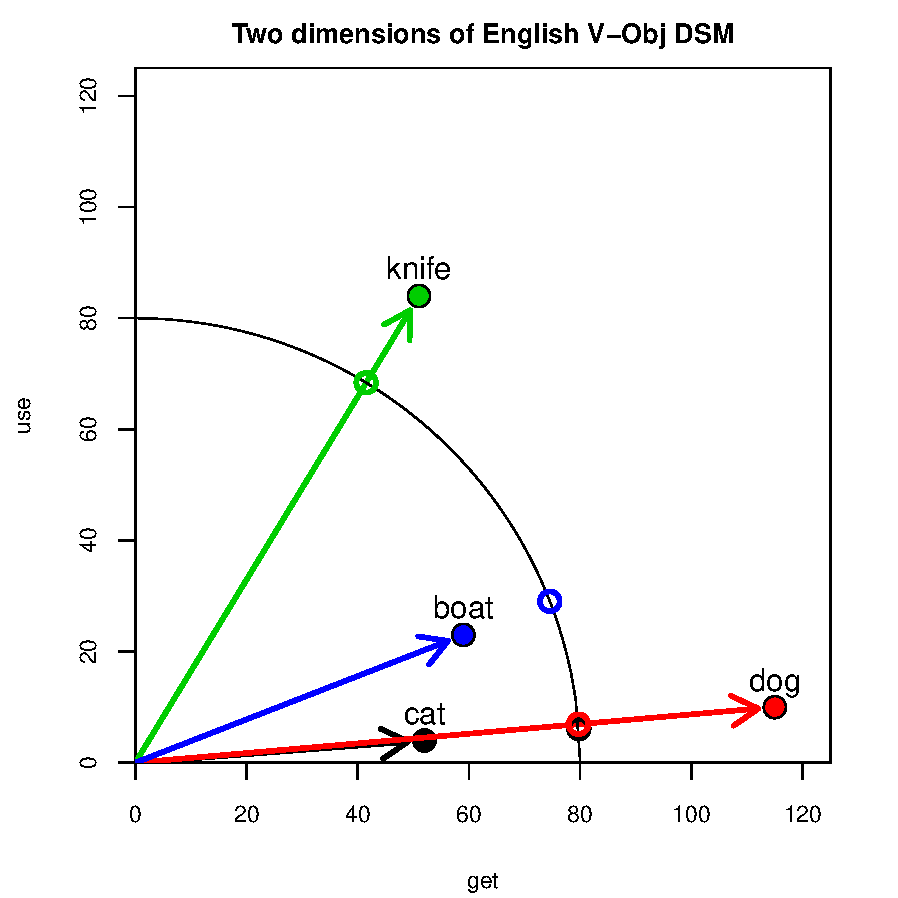
\includegraphics[width=6cm]{img/hieroglyph_2d_4}
    \end{column}
  \end{columns}
\end{frame}

\begin{frame}
  \frametitle{Scaling of column vectors}
  % \framesubtitle{}

  \begin{itemize}
  \item In statistical analysis and machine learning, features are
    usually \primary{centred} and \primary{scaled} so that
    \begin{align*}
      \text{mean} & \quad \mu = 0 \\
      \text{variance} & \quad \sigma^2 = 1
    \end{align*}
  \item In DSM research, this step is less common for columns of $\mathbf{M}$
    \begin{itemize}
    \item centring is a prerequisite for certain dimensionality
      reduction and data analysis techniques (esp.\ PCA)
    \item scaling may give too much weight to rare features
    \end{itemize}
    \pause
  \item $\mathbf{M}$ cannot be row-normalised and column-scaled at the
    same time (result depends on ordering of the two steps)
  \end{itemize}
\end{frame}

\begin{frame}
  \frametitle{Overview of DSM parameters}
  % \framesubtitle{}

  \ungap[1]
  \begin{center}
    Linguistic pre-processing (definition of terms)\\
    $\Downarrow$\\
    Term-context \vs\ term-term matrix\\
    $\Downarrow$\\
    Size \& type of context / structured \vs\ unstructered\\
    $\Downarrow$\\
    Geometric \vs\ probabilistic interpretation\\
    $\Downarrow$\\
    Feature scaling\\
    $\Downarrow$\\
    Normalisation of rows and/or columns\\
    $\Downarrow$\\
    \h{Similarity / distance measure}\\
    $\Downarrow$\\
    Compression
  \end{center}
\end{frame}

\begin{frame}
  \frametitle{Geometric distance}
  %% \framesubtitle{}

  \begin{columns}[T]
    \begin{column}{60mm}
      \begin{itemize}
      \item \h{Distance} between vectors $\vu, \vv \in \setR^n$ \so
        (dis)\h{similarity}
        \begin{itemize}
        \item $\vu = (u_1, \ldots, u_n)$
        \item $\vv = (v_1, \ldots, v_n)$
        \end{itemize}
      \item<2-> \h{Euclidean} distance $\dist[2]{\vu}{\vv}$
      \item<3-> ``City block'' \h{Manhattan} distance $\dist[1]{\vu}{\vv}$
      \item<4-> Both are special cases of the \h{Minkowski} $p$-distance
        $\dist[p]{\vu}{\vv}$ (for $p\in [1, \infty]$)
      \end{itemize}
    \end{column}
    \begin{column}{45mm}
      \includegraphics[width=45mm]{img/2_distance_examples}
    \end{column}
  \end{columns}
  \gap[.5]
  \only<beamer:2| handout:0>{%
    \[ \dist[2]{\vu}{\vv} \coloneq \sqrt{(u_1 - v_1)^2 + \dots + (u_n - v_n)^2} \] }
  \only<beamer:3| handout:0>{%
    \[ \dist[1]{\vu}{\vv} \coloneq \abs{u_1 - v_1} + \dots + \abs{u_n - v_n} \] }
  \only<beamer:4-| handout:1>{%
    \[ \dist[p]{\vu}{\vv} \coloneq \bigl(
    \abs{u_1 - v_1}^p + \dots + \abs{u_n - v_n}^p
    \bigr)^{1/p} \] }
  \only<beamer:5-| handout:1>{%
    \[ \dist[\infty]{\vu}{\vv} = \max \bigset{\abs{u_1 - v_1}, \ldots, \abs{u_n - v_n}} \] }
\end{frame}


\begin{frame}
  \frametitle{Other distance measures}
  % \framesubtitle{}
  
  \begin{itemize}
  \item Information theory: \h{Kullback-Leibler} (KL) \h{divergence} for probability vectors (non-negative, $\norm[1]{\vx} = 1$)
    \[
    \KL{\vu}{\vv} = \sum_{i=1}^n u_i \cdot \log_2 \frac{u_i}{v_i}
    \]
    \pause
  \item Properties of KL divergence
    \begin{itemize}
    \item most appropriate in a probabilistic interpretation of $\mathbf{M}$
    \item not symmetric, unlike all other measures
    \item alternatives: skew divergence, Jensen-Shannon divergence
    \end{itemize}
  \end{itemize}
\end{frame}

\begin{frame}
  \frametitle{Similarity measures}
  % \framesubtitle{}
  
  \begin{columns}[c]
    \begin{column}{5cm}
      \begin{itemize}
        \item angle $\alpha$ between two vectors $\vu,\vv$ is given by
          \begin{align*}
            \cos \alpha &= 
            \frac{\sum_{i=1}^n u_i\cdot v_i}{
              \sqrt{\sum_i u_i^2}\cdot \sqrt{\sum_i v_i^2}}
            \\
            &= \frac{\sprod{\vu}{\vv}}{\norm[2]{\vu}\cdot \norm[2]{\vv}}
        \end{align*}
      \item<2-> \h{cosine} measure of similarity: $\cos \alpha$
        \begin{itemize}
        \item $\cos \alpha = 1$ \so collinear
        \item $\cos \alpha = 0$ \so orthogonal
        \end{itemize}
      \end{itemize}
    \end{column}
    \begin{column}{6cm}
      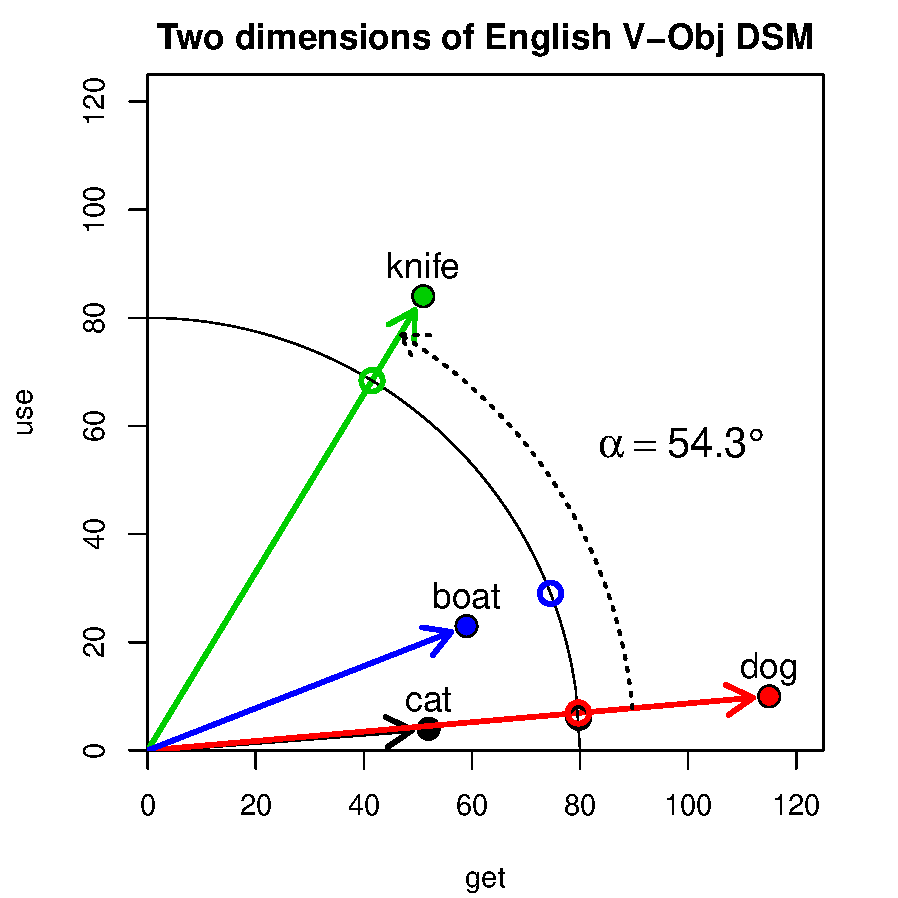
\includegraphics[width=6cm]{img/hieroglyph_2d_5}
    \end{column}
  \end{columns}
\end{frame}

\begin{frame}
  \frametitle{Overview of DSM parameters}
  % \framesubtitle{}

  \ungap[1]
  \begin{center}
    Linguistic pre-processing (definition of terms)\\
    $\Downarrow$\\
    Term-context \vs\ term-term matrix\\
    $\Downarrow$\\
    Size \& type of context / structured \vs\ unstructered\\
    $\Downarrow$\\
    Geometric \vs\ probabilistic interpretation\\
    $\Downarrow$\\
    Feature scaling\\
    $\Downarrow$\\
    Normalisation of rows and/or columns\\
    $\Downarrow$\\
    Similarity / distance measure\\
    $\Downarrow$\\
    \h{Compression}
  \end{center}
\end{frame}

\begin{frame}
  \frametitle{Model compression = dimensionality reduction}
  % \framesubtitle{}

  \begin{itemize}
  \item Co-occurrence matrix $\mathbf{M}$ is often unmanageably large\\
    and can be extremely sparse
    \begin{itemize}
    \item Google Web1T5: 1M $\times$ 1M matrix with one trillion
      cells, of which less than 0.05\% contain nonzero counts \citep{Evert:10a}
    \end{itemize}
  \item[\So] Compress matrix by reducing dimensionality (= rows)
    \begin{itemize}
    \item[]\pause
    \end{itemize}
  \item \h{Feature selection}: columns with high frequency \& variance
    \begin{itemize}
    \item measured by entropy, chi-squared test, \ldots
    \item may select correlated (\so uninformative) dimensions
    \item joint selection of multiple features is expensive
    \end{itemize}
    \pause
  \item \h{Projection} into (linear) subspace
    \begin{itemize}
    \item principal component analysis (PCA)
    \item independent component analysis (ICA)
    \item random indexing (RI)
    \item[\hand] intuition: preserve distances between data points
    \end{itemize}
  \end{itemize}
\end{frame}

\begin{frame}
  \frametitle{Dimensionality reduction \& latent dimensions}
  %% \framesubtitle{}

  \citet{Landauer:Dumais:97} claim that LSA dimensionality reduction (and related PCA technique) uncovers \h{latent dimensions} by exploiting correlations between features.

  \begin{columns}
    \begin{column}{6.5cm}
      \begin{itemize}
      \item Example: term-term matrix
      \item V-Obj cooc's extracted from BNC
        \begin{itemize}
        \item targets = noun lemmas\\
        \item features = verb lemmas
        \end{itemize}
      \item feature scaling: association scores (modified $\log$ Dice
        coefficient)
      \item $k=111$ nouns with $f \geq 20$\\
        (must have non-zero row vectors)
      \item $n=2$ dimensions: \emph{buy} and \emph{sell}
      \end{itemize}
    \end{column}
    \begin{column}{4cm}
      \begin{center}\footnotesize
        \begin{tabular}{l|rr}
          noun & \emph{buy} & \emph{sell} \\
          \hline
          \emph{bond}      &  0.28 &  0.77\\
          \emph{cigarette} & -0.52 &  0.44\\
          \emph{dress}     &  0.51 & -1.30\\
          \emph{freehold}  & -0.01 & -0.08\\
          \emph{land}      &  1.13 &  1.54\\
          \emph{number}    & -1.05 & -1.02\\
          \emph{per}       & -0.35 & -0.16\\
          \emph{pub}       & -0.08 & -1.30\\
          \emph{share}     &  1.92 &  1.99\\
          \emph{system}    & -1.63 & -0.70
        \end{tabular}
      \end{center}
    \end{column}
  \end{columns}
\end{frame}

\begin{frame}[c]
  \frametitle{Dimensionality reduction \& latent dimensions}
  %% \framesubtitle{}
  \begin{center}
    \ungap[1]
    \includegraphics[width=8cm]{img/3_buy_sell_labels_only}
  \end{center}
\end{frame}

\begin{frame}
  \frametitle{Motivating latent dimensions \& subspace projection}
  %% \framesubtitle{}

  \begin{itemize}
  \item The \h{latent property} of being a commodity is ``expressed''
    through associations with several verbs: \emph{sell}, \emph{buy},
    \emph{acquire}, \ldots
  \item Consequence: these DSM dimensions will be \h{correlated}
  \item[]\pause
  \item Identify \h{latent dimension} by looking for strong correlations\\
    (or weaker correlations between large sets of features)%
  \item Projection into subspace $V$ of $k < n$ latent dimensions\\
    as a ``\h{noise reduction}'' technique \so \hh{LSA}
  \item Assumptions of this approach:
    \begin{itemize}
    \item ``latent'' distances in $V$ are semantically meaningful
    \item other ``residual'' dimensions represent chance co-occurrence
      patterns, often particular to the corpus underlying the DSM
    \end{itemize}
  \end{itemize}
\end{frame}

\begin{frame}[c]
  \frametitle{The latent ``commodity'' dimension}
  %% \framesubtitle{}
  \begin{center}
    \ungap[1]
    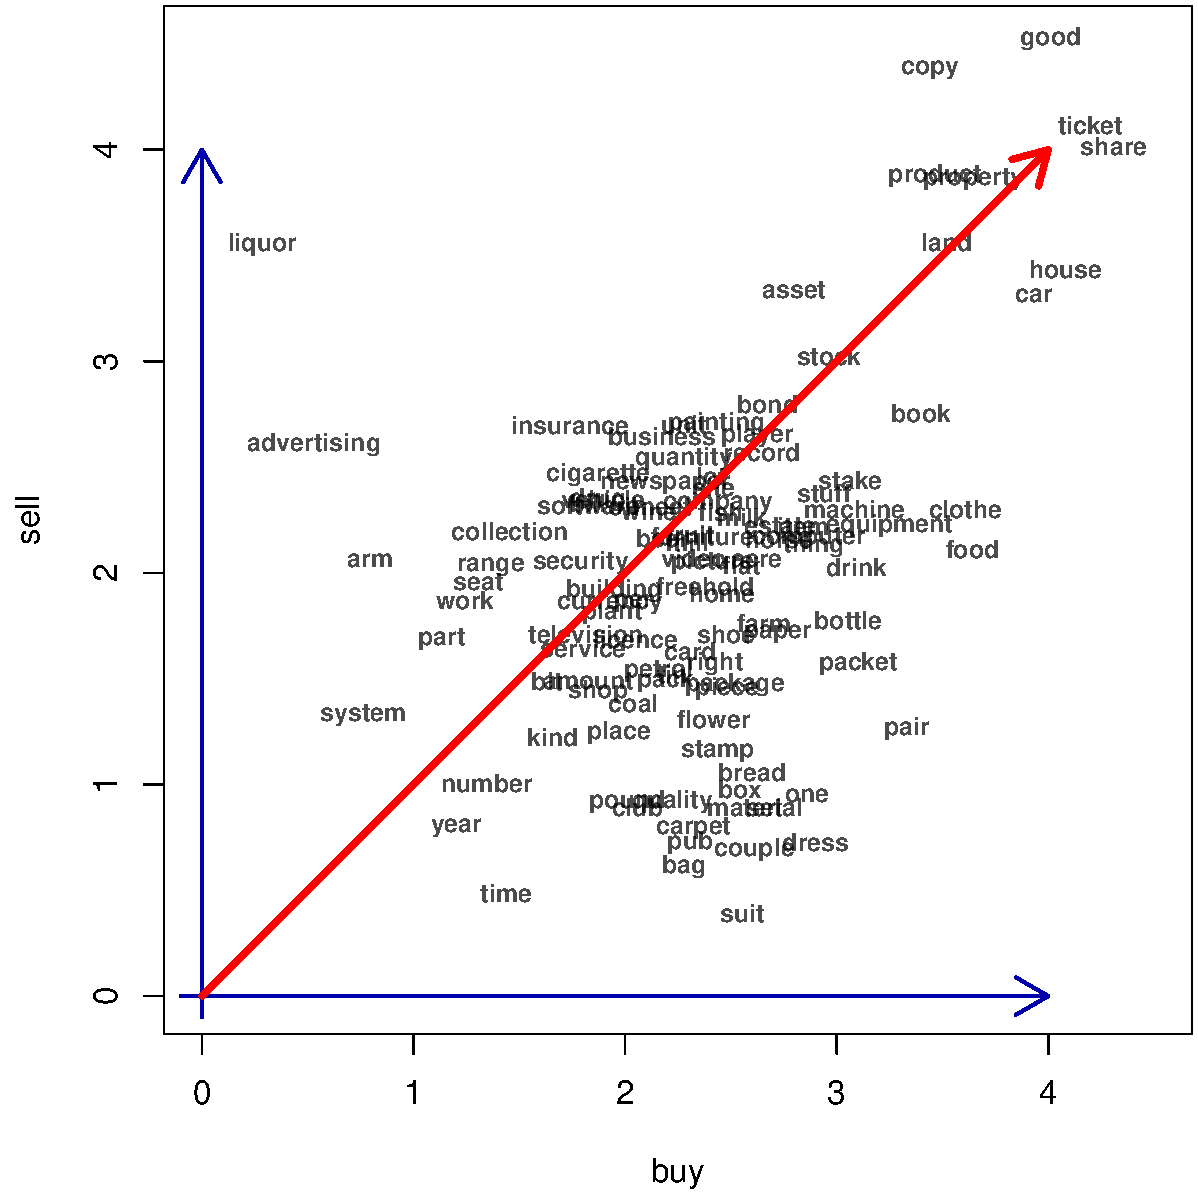
\includegraphics[width=8cm]{img/3_buy_sell_labels_latent}
  \end{center}
\end{frame}


%%%%%%%%%%%%%%%%%%%%%%%%%%%%%%%%%%%%%%%%%%
\subsection{Examples}

\begin{frame}
  \frametitle{Some well-known DSM examples}

  \ungap
  \begin{block} {Latent Semantic Analysis \citep{Landauer:Dumais:97}}
  \begin{itemize}
  \item term-context matrix with document context
  \item weighting: log term frequency and term entropy
  \item distance measure: cosine
  \item compression: SVD
  \end{itemize}
  \end{block}
 
 \begin{block} {Hyperspace Analogue to Language \citep{Lund:Burgess:96}}
  \begin{itemize}
  \item term-term matrix with surface context
  \item structured (left/right) and distance-weighted frequency counts
  \item distance measure: Minkowski metric ($1\leq p \leq 2$)
  \item compression: feature selection (high variance)
  \end{itemize}
  \end{block}
\end{frame}

\begin{frame}
  \frametitle{Some well-known DSM examples}

  \ungap
  \begin{block} {Infomap NLP \citep{Widdows:04}}
  \begin{itemize}
  \item term-term matrix with unstructured surface context
  \item weighting: none
  \item distance measure: cosine
  \item compression: SVD
  \end{itemize}
  \end{block}
 
  \begin{block} {Random Indexing (Karlgren \& Sahlgren 2001)}
    \begin{itemize}
    \item term-term matrix with unstructured surface context
    \item weighting: various methods 
    \item distance measure: various methods
    \item compression: random indexing (RI)
    \end{itemize}
  \end{block}
\end{frame}

\begin{frame}
  \frametitle{Some well-known DSM examples}

  \ungap
  \begin{block}{Dependency Vectors \citep{Pado:Lapata:07}}
  \begin{itemize}
  \item term-term matrix with unstructured dependency context
  \item weighting: log-likelihood ratio
  \item distance measure: information-theoretic \citep{Lin:98a}
  \item compression: none
  \end{itemize}
  \end{block}
 
 \begin{block} {Distributional Memory  (Baroni \& Lenci 2009)}
  \begin{itemize}
  \item both term-context and term-term matrices
  \item context: structured dependency context
  \item weighting: local-MI association measure
  \item distance measure: cosine
  \item compression: none
  \end{itemize}
  \end{block}
 \end{frame}


%%% Local Variables: 
%%% mode: latex
%%% TeX-master: "../workspace"
%%% End: 
